%% LyX 2.3.6.1 created this file.  For more info, see http://www.lyx.org/.
%% Do not edit unless you really know what you are doing.
\documentclass[english]{article}
\usepackage[T1]{fontenc}
\usepackage[latin9]{inputenc}
\usepackage{geometry}
\geometry{verbose,tmargin=2.5cm,bmargin=2.5cm,lmargin=2.5cm,rmargin=2.5cm}
\usepackage{calc}
\usepackage{graphicx}
\PassOptionsToPackage{normalem}{ulem}
\usepackage{ulem}

\makeatletter

%%%%%%%%%%%%%%%%%%%%%%%%%%%%%% LyX specific LaTeX commands.
%% Because html converters don't know tabularnewline
\providecommand{\tabularnewline}{\\}

\makeatother

\usepackage{babel}
\begin{document}
{[}SPLIT\_HERE{]}
\begin{enumerate}
\item \textbf{{[}ALVL/9597/2018/P1/Q1{]} }

A program is required to input and process the number of steps taken
by members of a walking club each week. The number of steps taken
by each member is an integer in the range 0 to 100000. 

Each week, the \textquotedblleft Star of the Week\textquotedbl{} is
the member who has taken the greatest number of steps. 

The name and number of steps taken by the \textbf{previous} week's
\textquotedbl Star of the Week\textquotedbl{} are stored in the text
file, \texttt{STAR.TXT}. 

The program specification is as follows: 
\begin{itemize}
\item Input \textbf{up to} 10 names and the number of steps each has taken.
Assume that each number of steps is unique. 
\item Find the walker who has taken the greatest number of steps from this
data. 
\item Read the data about the previous \textquotedblleft Star of the Week\textquotedblright{}
from the text file \texttt{STAR. TXT}. 
\item Display a message on screen to show the previous star of the week
\textbf{and} the new star of the week, each with their number of steps.
For example, 

\texttt{Last week, Jenny Smith was 'Star of the Week' with 75827 steps
taken. }

\texttt{This week, Vanessa Lim is 'Star of the Week' with 67152 steps
taken. }
\item Update the text file, \texttt{STAR.TXT}, with the details of the new
\textquotedbl Star of the Week\textquotedblright . 
\end{itemize}

\subsubsection*{Task 1.1}

Write program code for this task that includes validation of data
entered.

\subsubsection*{Evidence 1}

Your program code. \hfill{}{[}8{]}

The program needs to be tested with different test cases. Consider
carefully, test cases for input of names and steps. 

\subsubsection*{Task 1.2}

Copy the table with the following headings. Add other test cases to
the table. One type of test case has already been added to the table.
\begin{center}
\begin{tabular}{|l|l|l|}
\hline 
\hspace{0.05\columnwidth}\textbf{Test case} & \textbf{Purpose of test data} & \textbf{Expected results}\tabularnewline
\hline 
Yi Ling Aw, 10232 & Test the maximum of 10 values & 10 values entered and star of\tabularnewline
Ryan Batisah, 42231 & entered into the program. & the week is Vanessa Lim with\tabularnewline
Lee Casmir, 35020 &  & 67152 steps taken.\tabularnewline
Daniel Bennett, 60192 &  & \tabularnewline
Sarah Heng Chee, 29389 &  & \tabularnewline
Vanessa Lim, 67152 &  & \tabularnewline
Wong Yip, 53231 &  & \tabularnewline
Rin Xie, 34200 &  & \tabularnewline
Tin Wee, 49480 &  & \tabularnewline
David Bala, 32010 &  & \tabularnewline
\hline 
\end{tabular}
\par\end{center}

\subsubsection*{Evidence 2}

Completed table with other test cases added. \hfill{}{[}4{]}

\subsubsection*{Task 1.3}

Use \textbf{three} of the test cases in the table, and produce a screenshot
for each.

\subsubsection*{Evidence 2}

Three screenshots of test cases.\hfill{}{[}3{]}

{[}SPLIT\_HERE{]}
\item \textbf{{[}ALVL/9597/2018/P1/Q2{]} }

The following algorithm is an implementation of a quick sort that
operates on an array \texttt{Scores}. 

This algorithm assumes that the first element of an array is the zeroth
element. This means that \texttt{Scores{[}0{]}} is the first element
in the array.

This pseudocode is available in the file \texttt{QUICKSORT.TXT}

\noindent\begin{minipage}[t]{1\columnwidth}%
\noindent \texttt{FUNCTION QuickSort(Scores)}

\noindent \texttt{\qquad{}QuickSortHelper(Scores, 0, LENGTH(Scores)
- 1)}

\noindent \texttt{\qquad{}RETURN Scores}

\noindent \texttt{ENDFUNCTION}

\bigskip{}

\noindent \texttt{FUNCTION QuickSortHelper(Scores, First, Last)}

\noindent \texttt{\qquad{}IF First < Last}

\noindent \texttt{\qquad{}THEN}

\noindent \texttt{\qquad{}\qquad{}SplitPoint <- PartitioniScores,
First, Last)}

\noindent \texttt{\qquad{}\qquad{}QuickSortHelper(Scores, First,
SplitPoint \textemdash{} 1)}

\noindent \texttt{\qquad{}\qquad{}QuickSoRtHelper(Scores, SplitPoint
+ 1, Last)}

\noindent \texttt{\qquad{}ENDIF}

\noindent \texttt{\qquad{}RETURN Scores}

\noindent \texttt{ENDFUNCTION }\bigskip{}

\noindent \texttt{FUNCTION Partition(Scores, First, Last)}

\noindent \texttt{\qquad{}PivotValue <- ScoresiFirst{]}}

\noindent \texttt{\qquad{}Lefthark <- First + 1}

\noindent \texttt{\qquad{}RightMark <- Last}

\noindent \texttt{\qquad{}Done <- FALSE}

\noindent \texttt{\qquad{}WHILE (Done = FALSE)}

\noindent \texttt{\qquad{}\qquad{}WHILE LeftMark <= RightMark AND
Scores{[}LeftMark{]} <= PivotValue}

\noindent \texttt{\qquad{}\qquad{}\qquad{}LeftMark <- LeftMark
+ 1}

\noindent \texttt{\qquad{}\qquad{}ENDWHILE}

\noindent \texttt{\qquad{}\qquad{}WHILE Scores{[}RightMark{]} >=
PivotValue AND RightMark >= LeftMark}

\noindent \texttt{\qquad{}\qquad{}\qquad{}RightMark <- RightMark
\textemdash{} 1}

\noindent \texttt{\qquad{}\qquad{}ENDWHILE}

\noindent \texttt{\qquad{}\qquad{}IF RightMark < LeftMark}

\noindent \texttt{\qquad{}\qquad{}\qquad{}THEN}

\noindent \texttt{\qquad{}\qquad{}\qquad{}\qquad{}Done <- TRUE}

\noindent \texttt{\qquad{}\qquad{}ELSE}

\noindent \texttt{\qquad{}\qquad{}\qquad{}Temp <- Scores{[}LeftMark{]}}

\noindent \texttt{\qquad{}\qquad{}\qquad{}Scores{[}LeftMark{]}
<- Scores{[}RightMark{]}}

\noindent \texttt{\qquad{}\qquad{}\qquad{}Scores{[}RightMark{]}
<- Temp}

\noindent \texttt{\qquad{}ENDIF}

\noindent \texttt{ENDWHILE }\bigskip{}

\noindent \texttt{\textbf{\emph{<swap Scores{[}First{]} with Scores{[}RightMark{]}>}}}\texttt{
}\bigskip{}

\noindent \texttt{\qquad{}RETURN RightMark}

\noindent \texttt{ENDFUNCTION}%
\end{minipage}

\subsubsection*{Task 2.1}

Write program code to implement this algorithm. Ensure that you add
the missing code to complete the algorithm. The area of missing code
is highlighted as:
\begin{center}
\texttt{\textbf{\emph{<swap Scores {[}First{]} with Scores {[}RightMark{]}>}}}
\par\end{center}

Copy the sample data available in the \texttt{SCORES.TXT} file. Paste
this into your programming code to set up the data to be sorted.

\subsubsection*{Evidence 4}

Your program code. \hfill{}{[}12{]}

\subsubsection*{Task 2.2}

Add a function to your code to output Scores. Call this function before
and after the operation of the quick sort so that the unsorted and
sorted data is displayed.

\subsubsection*{Evidence 5}

Your program code. \hfill{}{[}2{]}

\subsubsection*{Evidence 6}

Screenshot showing the unsorted and sorted \texttt{Scores} data.\hfill{}
{[}1{]}

{[}SPLIT\_HERE{]}
\item \textbf{{[}ALVL/9597/2018/P1/Q3{]} }

The file,\texttt{ HASHEDDATA.TXT}, holds details of the names and
telephone numbers of 250 people. 

There are a total of 500 lines in the file, and a number of these
lines are empty of name and telephone number.

An index is stored for each line of the file. 

The format of the data in the file is: 
\begin{center}
<Index>,<PersonName>,<TelephoneNumber> 
\par\end{center}

The first 10 lines from the file are shown as follows: 

\noindent\fbox{\begin{minipage}[t]{1\columnwidth - 2\fboxsep - 2\fboxrule}%
0, ,

1, ,

2, ,

3, Boon Keng V., 07492 546415

4, ,

5, ,

6, Ahmad Yusof, 07439 778665

7, Durno Peter, 07662 863518

8, Batisah Wong, 07362 156265

9, ,%
\end{minipage}}

The values in the file are separated by the comma character. 

A record structure is used to store a name and telephone number. A
data structure of 500 records is needed to store all the names and
telephone numbers. Each line in the file is written to a corresponding
position in the data structure.

The records with index six to eight from the data structure are: 
\begin{center}
\begin{tabular}{r|c|c|}
\cline{2-3} \cline{3-3} 
\textbf{Index} & \textbf{PersonName} & \textbf{TelephoneNumber}\tabularnewline
\cline{2-3} \cline{3-3} 
6 & Ahmad Yusof & 07439 778665\tabularnewline
\cline{2-3} \cline{3-3} 
7 & Durno Peter & 07662 863518\tabularnewline
\cline{2-3} \cline{3-3} 
\texttt{8} & Batisah Wong & 07362 156265\tabularnewline
\cline{2-3} \cline{3-3} 
\end{tabular}
\par\end{center}

\subsubsection*{Task 3.1}

Use program code to create a:
\begin{itemize}
\item record structure to hold the name and telephone number for one person
\item data structure, using this record structure to store 500 records.
\end{itemize}

\subsubsection*{Evidence 7}

Your program code. \hfill{}{[}6{]}

\subsubsection*{Task 3.2}

Write program code to:
\begin{itemize}
\item read the lines from the file
\item extract the <Index>, <PersonName> and <TelephoneNumber> values
\item store these values in the data structure.
\end{itemize}
Create a procedure called \texttt{DisplayValues} that will loop though
the data structure and display the index, name and telephone number
for every record where the name is present.

Ensure your procedure uses headings to identify the data displayed.

\subsubsection*{Evidence 8}

Your program code. \hfill{}{[}13{]}

\subsubsection*{Evidence 9}

A Screenshot showing the output.\hfill{} {[}1{]}

A hashing function was used to create the file. The same hashing function
can be used to search the data structure for a particular name. The
hashing function generates a hash. This is calculated as follows:

\noindent\begin{minipage}[t]{1\columnwidth}%
\texttt{Get SearchName}

\texttt{Set HashTotal to 0}

\texttt{FOR each Character in SearchName}

\texttt{\qquad{}Get the ASCII code for Character}

\texttt{\qquad{}Multiply the ASCII code by the position of Character
in SearchName}

\texttt{\qquad{}Add the result to the HashTotal}

\texttt{Calculate Hash as HashTotal MOD 500}

\texttt{RETURN Hash}%
\end{minipage}

\subsubsection*{Task 3.3}

Add the program code for the hashing function. Use the following specification:
\begin{center}
\texttt{FUNCTION GenerateHash(SearchName : STRING) : INTEGER}
\par\end{center}

The function has a single parameter \texttt{SearchName} and returns
an integer value.

Write additional code for your program to allow you to test the implementation
of this function.

The following test data will assist you.

\qquad{}\textquotedblleft Tait Davinder\textquotedblright{} should
return a hash of 87

\qquad{}\textquotedblleft Anandan Yeo\textquotedbl{} should return
a hash of 156

\subsubsection*{Evidence 10}

Your program code. \hfill{}{[}8{]}

\subsubsection*{Evidence 11}

A screenshot (or screenshots) of your program to show the results
of the hash calculation for both the given test data values.\hfill{}{[}2{]}

The hash calculated from the \texttt{SearchName} can be used to find
a corresponding record in the data structure.

If the \texttt{SearchName} is not found in the record given by the
hash \textbf{and} the record is not empty:
\begin{itemize}
\item compare \texttt{SearchName} with the next record
\item until the \texttt{SearchName} is found or an empty record is found.
\end{itemize}
If an empty record is found then the program will report that the
name is \textquotedblleft NOT FOUND\textquotedblright .

If the record is found, the program will output the index, name and
telephone number.

\subsubsection*{Task 3.4}

Add the program code to implement the search as described.

\subsubsection*{Evidence 12}

Your program code. \hfill{}{[}7{]}

\subsubsection*{Evidence 11}

A screenshot (or screenshots) of your program to show the results
of the following searches:

Search 1: Charlie Love

Search 2: Chin Tan

Search 3: John Barrowman\hfill{}{[}3{]}

{[}SPLIT\_HERE{]}
\item \textbf{{[}ALVL/9597/2018/P1/Q4{]} }

In a computer game, a player (\textquotedbl\texttt{O}\textquotedbl )
moves around a maze measuring 10 metres by 11 metres to collect a
prize (\textquotedbl\texttt{P}\textquotedbl ). The prize is placed
at a random position within the maze. The prize position is not where
a wall (\textquotedbl\texttt{X}\textquotedbl ) appears in the maze.
An empty position is indicated with a full-stop (\textquotedbl\texttt{.}\textquotedbl ). 

The maze is represented on the screen by a rectangular grid. Each
square metre of the maze is represented by an x-coordinate and a y-coordinate.
The top left square metre of the puzzle display has x = \texttt{0}
and y = \texttt{0}.

The player moves left, right, up or down according to a direction
entered by the user. The game is turn-based; a user enters the direction,
their player moves one position in that direction. lithe direction
would place the player on a well, then the player does not move. The
maze is displayed after each move.
\begin{center}
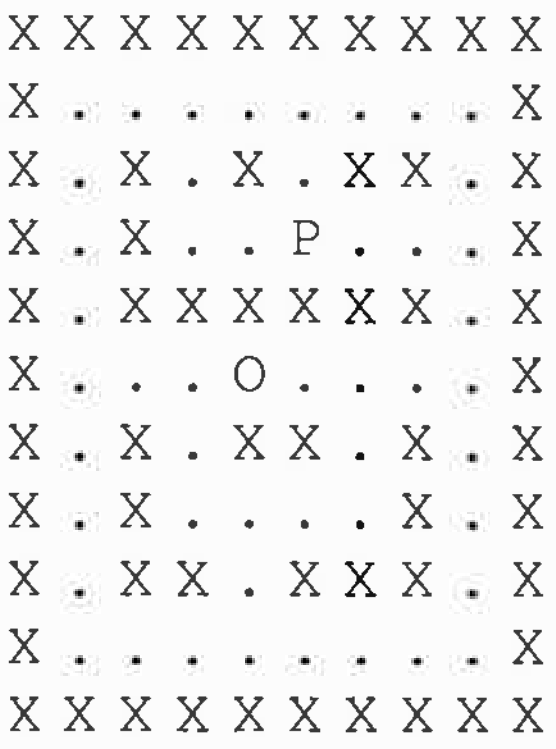
\includegraphics[width=0.25\paperwidth]{C:/Users/Admin/Desktop/Github/question_bank/LyX/static/img/9597-ALVL-2018-P1-Q4}
\par\end{center}

\subsubsection*{Task 4.1}

Write a program to display the maze as shown.
\begin{itemize}
\item The maze should be stored in a suitable data structure.
\item The data structure will allow fixed loop(s) to be used to display
the maze.
\end{itemize}
The maze is given in the text file \texttt{MAZE.TXT}. You may read
in the data from this file or place the data in your program using
any suitable method.

\subsubsection*{Evidence 14}

Your program code. \hfill{} {[}6{]}

\subsubsection*{Task 4.2}

The prize is placed randomly on the maze. It cannot appear in the
same grid position as a wall (\textquotedbl\texttt{X}\textquotedbl ).

Add to your program code to place the prize at a random position.

Take a screenshot of the maze with the prize displayed in it.

\subsubsection*{Evidence 15}

Your program code. \hfill{}{[}4{]}

\subsubsection*{Evidence 16}

A screenshot of the maze as output by your program. \hfill{} {[}1{]}

The player is represented by the character \textquotedbl\texttt{O}\textquotedbl .
The character starts the game in a central position on the grid, for
example, x = \texttt{4} and y = \texttt{5}. 

To move the character, the user is prompted for a direction. The following
are valid inputs:
\begin{center}
\begin{tabular}{|c|l|}
\hline 
\textbf{Input character} & \hspace{0.05\columnwidth}\textbf{Action}\tabularnewline
\hline 
\texttt{``U''} & Player moves up\tabularnewline
\hline 
\texttt{``D''} & Player moves down\tabularnewline
\hline 
\texttt{``L''} & Player moves left\tabularnewline
\hline 
\texttt{``R''} & Player moves right\tabularnewline
\hline 
\texttt{``''} & Continue with previous move.\tabularnewline
 & If no previous move, do nothing\tabularnewline
\hline 
\end{tabular}
\par\end{center}

If the next position for the player (\textquotedbl\texttt{O}\textquotedbl )
is a wall (\textquotedbl\texttt{X}\textquotedbl ), then the player
stays in their current position; this is called collision detection.

When the player enters the move, a new position for the player (\textquotedbl\texttt{O}\textquotedbl )
is calculated and the maze is displayed. The previous position is
changed back to a \textquotedbl .\textquotedbl{} when the player
has a new position. The moves are repeated until the player is at
the same position as the prize.

\subsubsection*{Task 4.3}

Add to your program code to:
\begin{itemize}
\item place the player on the grid at a central position on the grid
\item take in and validate a direction
\item calculate a new position
\item check this position is not a wall
\item update the grid so that the previous position of \textquotedbl\texttt{O}\textquotedbl{}
is replaced with a \textquotedbl{} . \textquotedbl{} and \textquotedbl\texttt{O}\textquotedbl{}
is located in its new position
\item continue this until the player is at the same position as the prize.
\end{itemize}

\subsubsection*{Evidence 17}

Your program code. \hfill{} {[}16{]}

When the player and the prize are at the same position, the message
\textquotedblleft Player has reached the prize\textquotedblright{}
is displayed and the game ends.

\subsubsection*{Task 4.4}

Add to your program, code to end the game when this condition is met,
and display the required message. Produce screenshots to show key
elements of your program are functioning.

The screenshots required are:
\begin{itemize}
\item entering each direction
\item player changing position
\item end of game
\end{itemize}

\subsubsection*{Evidence 18}

Your program code. \hfill{} {[}1{]}

\subsubsection*{Evidence 19}

Screenshots of:
\begin{itemize}
\item entering each direction
\item player changing position
\item end of game (player wins) \hfill{} {[}2{]}
\end{itemize}
{[}SPLIT\_HERE{]}
\item \textbf{{[}ALVL/9597/2018/P2/Q1{]} }

A mobile phone company has an option for Pay As You Go usage. Customers
have to purchase credit in advance. The credit is used to pay for
texts, calls and data. Customers can buy additional credit at any
time. 

The company requires software to allow their Pay As You Go customers
to do the following tasks online: 
\begin{itemize}
\item check credit balance 
\item check data usage 
\item check call usage 
\item pay for credit 
\end{itemize}
A software company was employed to put together a project team to
produce the software. 
\begin{enumerate}
\item State \textbf{three} members of the project team. Describe the role
of each of these members. \hfill{}{[}6{]}
\item The initial phase of the system development cycle required that a
specification be created for the system. 
\begin{enumerate}
\item State \textbf{two} techniques that could have been used to gather
the information for this specification. \hfill{} {[}2{]}
\item Explain how each technique would have been used in this project. \hfill{}
{[}4{]}
\end{enumerate}
\item The specification is a detailed report.

Describe \textbf{two} sections of this report. \hfill{}{[}4{]}
\item The software could have been designed using different techniques. 
\begin{enumerate}
\item Name \textbf{and} describe \textbf{two} design techniques that may
have been used. \hfill{} {[}4{]}
\item Explain why it is important for each member of the design team to
use the same technique. \hfill{} {[}2{]}
\item A customer's mobile phone number needs to be validated on entry. 

Draw a flowchart to represent an algorithm for this validation. \hfill{}
{[}4{]}
\end{enumerate}
\item (e) The work to implement the new software needs to be managed. The
following Program Evaluation and Review Technique (PERT) chart is
used as a management tool. 

\texttt{A} --- Specification 

\texttt{B} --- Analysis 

\texttt{C} --- Design of software 

\texttt{D} --- Design of Interface 

\texttt{E} --- Documentation 

\texttt{F}--- Implementation 

\texttt{G} --- Testing 

\texttt{H} --- Acceptance testing

\texttt{I} --- Hand over to phone company 

Time is measured in weeks. 
\begin{center}
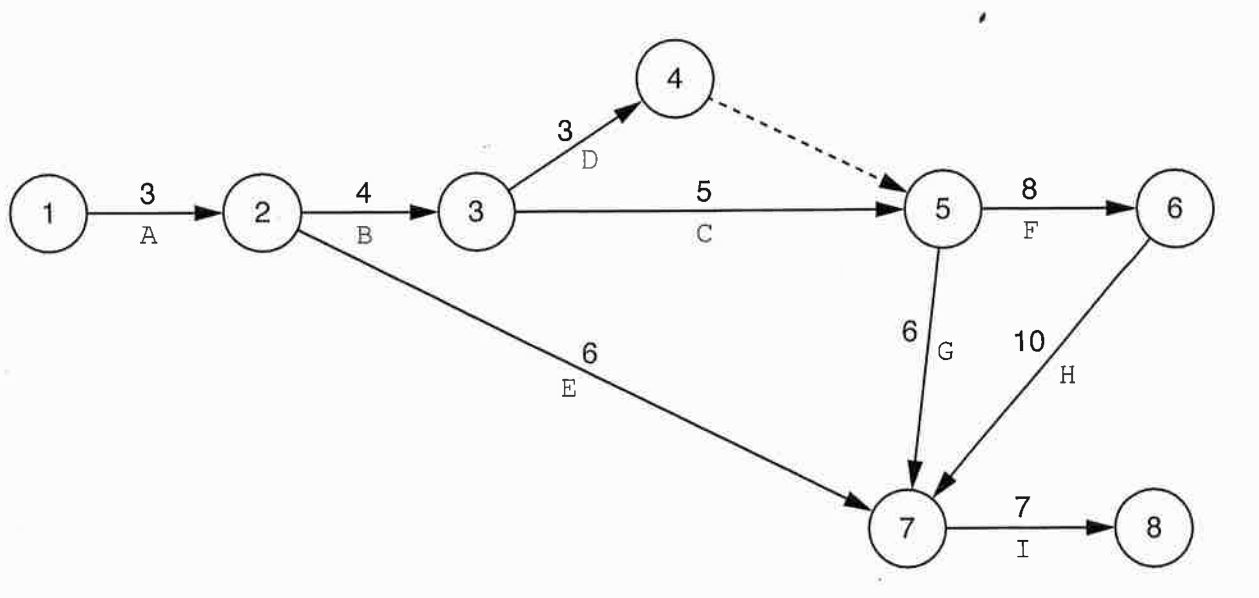
\includegraphics[width=0.5\paperwidth]{C:/Users/Admin/Desktop/Github/question_bank/LyX/static/img/9597-ALVL-2018-P2-Q1}
\par\end{center}
\begin{enumerate}
\item State the critical path for the given activities \texttt{A} to \texttt{I}.
\hfill{}{[}2{]}
\item Calculate the minimum time these activities will take. \hfill{}{[}1{]}
\item The member of the project team who worked on activity 0 fold the project
manager he could not start work until one week after the scheduled
start date. 

Explain any impact this would have on the completion date of the project.\hfill{}
{[}3{]}
\end{enumerate}
\item The software is intended for use on hand-held devices. 

Describe \textbf{two} ways that users can keep their data secure on
these devices.\hfill{} {[}4{]}
\item A member of the project team had the task of ensuring that social
and ethical issues were considered. 

Describe \textbf{one} example of each of these Issues that this member
of the team might have considered. \hfill{}{[}4{]}
\end{enumerate}
{[}SPLIT\_HERE{]}
\item \textbf{{[}ALVL/9597/2018/P2/Q2{]} }

The following algorithm calculates the average mark for a group of
students. 

\noindent\begin{minipage}[t]{1\columnwidth}%
\texttt{01 FOR Counter <- 1 TO NumberOfStudents}

\texttt{02 \qquad{}Total <- O}

\texttt{03 \qquad{}INPUT Mark}

\texttt{04 \qquad{}Total <- Total + Mark}

\texttt{05 ENDFOR}

\texttt{06 Average <- Total / NumberOfStudents}

\texttt{07 OUTPUT Average}%
\end{minipage}
\begin{enumerate}
\item There is an error in this algorithm causing an incorrect result. Describe
the error and explain the change required to correct this error. \hfill{}{[}3{]}
\item State the name of this type of error.\hfill{} {[}1{]}
\item The lowest mark in the exam is 0 and the highest is 100. Give an example
from each of the appropriate test cases which could be used to test
the algorithm. \hfill{}{[}4{]}
\item Name and describe a suitable technique that could be used to manually
identify errors in the algorithm. \hfill{}{[}2{]}
\end{enumerate}
{[}SPLIT\_HERE{]}
\item \textbf{{[}ALVL/9597/2018/P2/Q3{]} }
\begin{enumerate}
\item A binary tree is as follows: 
\begin{center}
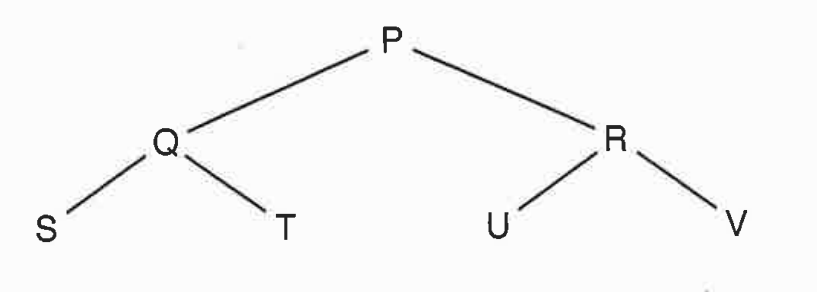
\includegraphics[width=0.5\paperwidth]{C:/Users/Admin/Desktop/Github/question_bank/LyX/static/img/9597-ALVL-2018-P2-Q3}
\par\end{center}
\begin{enumerate}
\item State the in-order sequence. \hfill{}{[}1{]}
\item State the pre-order sequence. \hfill{} {[}1{]}
\end{enumerate}
\item A 1D array, \texttt{Value}, stores a list of scores as follows:
\begin{center}
\begin{tabular}{|c|c|c|c|c|c|c|c|c|c|c|c|c|c|c|c|}
\hline 
Index & 0 & 1 & 2 & 3 & 4 & 5 & 6 & 7 & 8 & 9 & 10 & 11 & 12 & 13 & 14\tabularnewline
\hline 
Score & 2 & 6 & 15 & 23 & 36 & 48 & 50 & 58 & 64 & 69 & 74 & 79 & 86 & 92 & 99\tabularnewline
\hline 
\end{tabular}
\par\end{center}
\begin{enumerate}
\item Using a linear search, state how many comparisons will be required
to find the score of 64. \hfill{}{[}1{]}
\end{enumerate}
The following binary search algorithm could be used to search the
list of scores.

\noindent\begin{minipage}[t]{1\columnwidth}%
\texttt{01 Lower <- LowestIndex}

\texttt{02 Upper <- HighestIndex}

\texttt{03 REPEAT}

\texttt{04 \qquad{}Middle <- (Lower + Upper) DIV 2}

\texttt{05 \qquad{}IF SearchItem > Value{[}Middle{]}}

\texttt{O6 \qquad{}THEN}

\texttt{07 \qquad{}\qquad{}Lower <- Middle + l}

\texttt{08 \qquad{}ELSE}

\texttt{09 \qquad{}\qquad{}Upper <- Middle \textemdash{} l}

\texttt{10 \qquad{}ENDIF}

\texttt{11 UNTIL Value{[}Middle{]} = SearchItem OR Lower > Upper}

\texttt{12 OUTPUT \textquotedbl Score found at position\textquotedbl{}
Middle}%
\end{minipage}
\begin{enumerate}
\item[ii.] Score 80 is not in the list.

When searching for this score, state the values that will be examined.
\hfill{}{[}2{]}
\item[iii.] When searching for a score of 80, this algorithm outputs:

\texttt{Score found at position 12}

Describe how the algorithm gives this incorrect output. \hfill{}{[}2{]}
\item[iv.] Describe how the algorithm could be changed to give a suitable message
if the score is not in the list. \hfill{}{[}3{]}
\end{enumerate}
\end{enumerate}
{[}SPLIT\_HERE{]}
\item \textbf{{[}ALVL/9597/2018/P2/Q4{]} }

A university allows students to access the university network from
home. 
\begin{enumerate}
\item The university server has a firewall.

Describe \textbf{two} ways that a firewall can be used to block unauthorised
access to the network. \hfill{}{[}2{]}
\item The university wishes to restrict access to inappropriate websites
from within its network.

Describe \textbf{two} methods that could be used to restrict access
to inappropriate websites. \hfill{}{[}4{]}
\item The university is concerned about the possible loss of data from their
local servers.

Describe a strategy that could be used to prevent data loss. \hfill{}{[}2{]}
\item The university has its own intranet.

Describe \textbf{two} benefits that the intranet might provide for
students. \hfill{}{[}2{]}
\end{enumerate}
{[}SPLIT\_HERE{]}
\item \textbf{{[}ALVL/9597/2018/P2/Q5{]} }

The organisers of a diving championship have created software to calculate
and show the total score for each diver. 

There are nine judges scoring each dive. The two best scores and the
two worst scores are ignored. The other five scores are added together
to give the diver\textquoteright s total score. 
\begin{enumerate}
\item Write an algorithm to take in the nine scores, delete the best two
and the two worst scores, and total the five remaining scores. \hfill{}{[}4{]}
\end{enumerate}
There are 10 divers in the final. The scoreboard shows the order of
diving. 
\begin{center}
\begin{tabular}{|c|c|l|}
\hline 
\textbf{Order} & \textbf{Diver name} & \textbf{Total score}\tabularnewline
\hline 
1 & Daniel Tan & \tabularnewline
\hline 
2 & Parker Lam & \tabularnewline
\hline 
3 & Mohamed Noor & \tabularnewline
\hline 
4 & Hariz Yazid & \tabularnewline
\hline 
5 & Sheryl Xuan & \tabularnewline
\hline 
6 & Karl Lim & \tabularnewline
\hline 
7 & Elaine Ning & \tabularnewline
\hline 
8 & Nadyia Esmadi & \tabularnewline
\hline 
9 & Cai Ng & \tabularnewline
\hline 
10 & Hamid Mahmood & \tabularnewline
\hline 
\end{tabular}
\par\end{center}
\begin{enumerate}
\item The programmers decided to use a 1D array for the scores. They will
also use a bubble sort to sort the scores into descending order.
\begin{enumerate}
\item Explain how a bubble sort can be used to arrange the scores into a
descending or ascending order. \hfill{}{[}2{]}
\end{enumerate}
This is the bubble sort algorithm for sorting into descending order:

\noindent\begin{minipage}[t]{1\columnwidth}%
\texttt{01 WHILE NoSwaps = FALSE}

\texttt{02 \qquad{}NoSwaps <- TRUE}

\texttt{03 \qquad{}UpperBound <- ListLength}

\texttt{04 \qquad{}FOR Posn <- 0 TO ......}\texttt{\textbf{A}}\texttt{......}

\texttt{05 \qquad{}\qquad{}IF List{[}Posn{]} < ......}\texttt{\textbf{B}}\texttt{......}

\texttt{06 \qquad{}\qquad{}\qquad{}THEN}

\texttt{O7 \qquad{}\qquad{}\qquad{}\qquad{}// Swap}

\texttt{O8 \qquad{}\qquad{}\qquad{}\qquad{}NoSwaps <- ......}\texttt{\textbf{C}}\texttt{......}

\texttt{09 \qquad{}\qquad{}\qquad{}\qquad{}Temp <- List{[}Posn{]}}

\texttt{10 \qquad{}\qquad{}\qquad{}\qquad{}List{[}Posn{]} <- ListiPosn
+ 1{]}}

\texttt{11 \qquad{}\qquad{}\qquad{}\qquad{}List{[}Posn + 1{]}
<- ......}\texttt{\textbf{D}}\texttt{......}

\texttt{12 \qquad{}\qquad{}ENDIF}

\texttt{l3 \qquad{}ENDFOR}

\texttt{14 ENDWHILE}%
\end{minipage}
\begin{enumerate}
\item Write the pseudocode for \texttt{\textbf{A}}, \texttt{\textbf{B}},
\texttt{\textbf{C}}\textbf{ a}nd \texttt{\textbf{D}} in the algorithm.
\hfill{} {[}4{]}
\end{enumerate}
\item During the first round of dives, the sorted scores for five divers
are: 

\texttt{48 }

\texttt{45 }

\texttt{40 }

\texttt{37 }

\texttt{36 }

The sixth diver scores 42 and the software appends the score to the
list as follows: 

\texttt{48 }

\texttt{45 }

\texttt{40 }

\texttt{37 }

\texttt{36 }

\texttt{42}
\begin{enumerate}
\item State the number of passes needed through the list to return the list
to its sorted order. \hfill{}{[}1{]}
\item Explain why the bubble sort is efficient in this example. \hfill{}{[}2{]}
\item Name another sort method that could have been used in this situation. 

Compare the speed of sorting the divers\textquoteright{} scores in
your named method with using the bubble sort. \hfill{}{[}2{]}
\end{enumerate}
\end{enumerate}
{[}SPLIT\_HERE{]}
\item \textbf{{[}ALVL/9597/2018/P2/Q6{]} }

Customers want to buy tickets for a diving championship that takes
place over three days. There are two sessions of diving each day. 

Customers use a ticket ordering website to buy their tickets.
\begin{center}
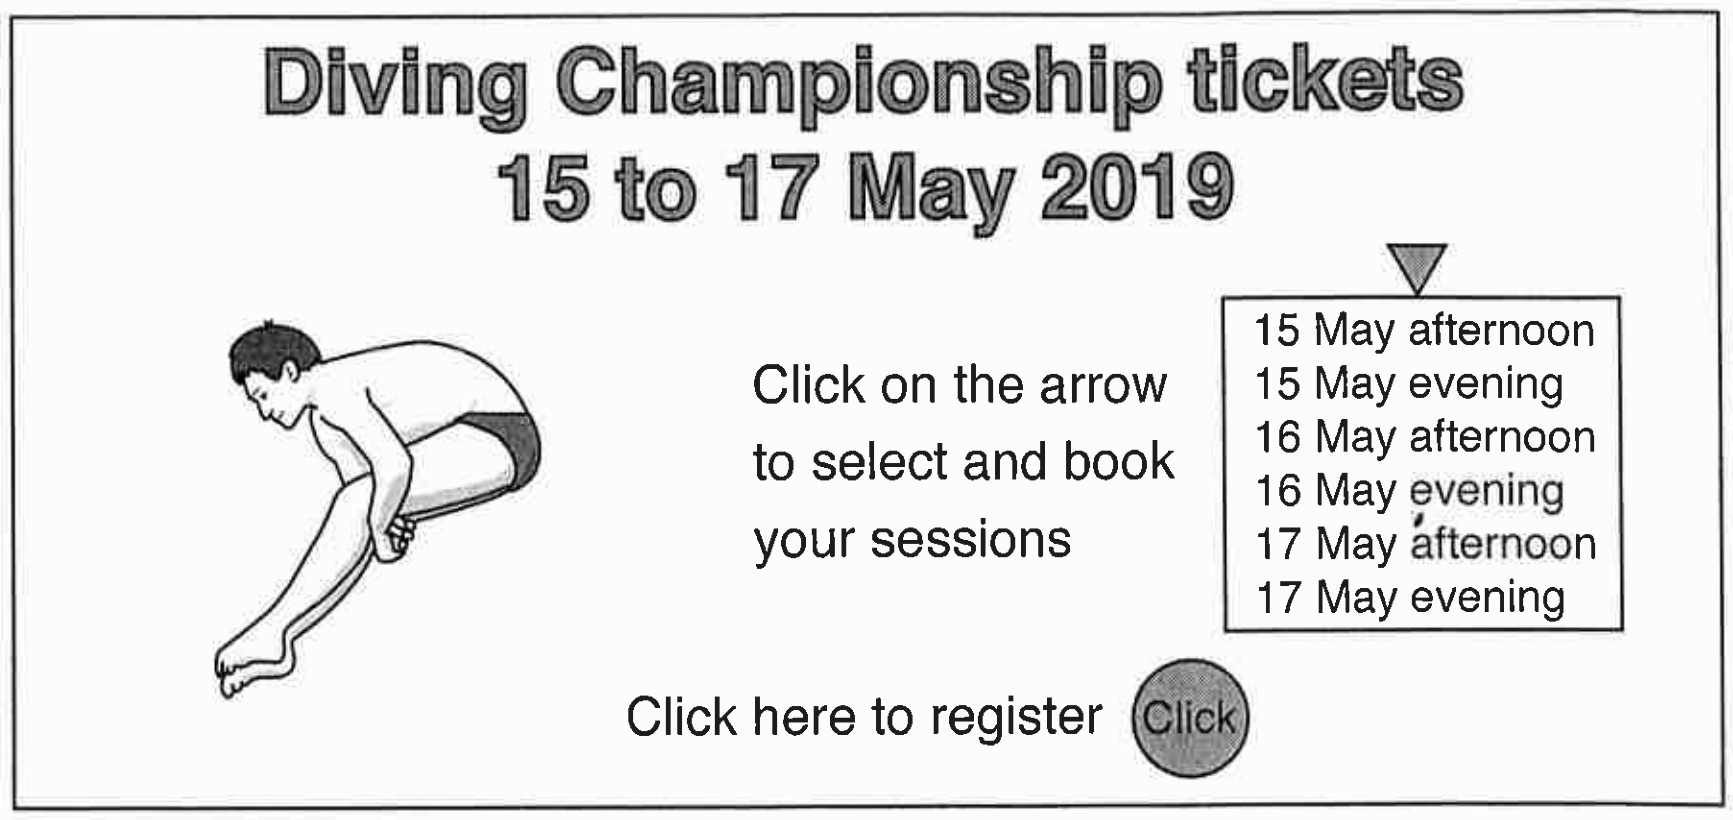
\includegraphics[width=0.5\paperwidth]{C:/Users/Admin/Desktop/Github/question_bank/LyX/static/img/9597-ALVL-2018-P2-Q6-1}
\par\end{center}
\begin{enumerate}
\item State the type of user interface that the ticket ordering website
uses. \hfill{}{[}1{]}
\item All ticket sales are stored on a database server in the following
tables: 

\texttt{CUSTOMER(}\texttt{\uline{CustomerID}}\texttt{, CustomerName,
Email, ContactNumber) }

\texttt{BOOKING(}\texttt{\uline{BookinoID}}\texttt{, BookingDate,
CustomerID) }

\texttt{SESSION(}\texttt{\uline{SessionID}}\texttt{, Date, Time,
SessionCost) }

\texttt{BOOKING\_SESSION(}\texttt{\uline{BookingID}}\texttt{, }\texttt{\uline{SessionID}}\texttt{,
Quantity)} 

\texttt{CustomerID} is the unique identifier in the \texttt{CUSTOMER}
table. 

\texttt{BookingID} is the unique identifier in the \texttt{BOOKING}
table. 

\texttt{SessionID} is the unique identifier in the \texttt{SESSION}
table. 
\begin{enumerate}
\item Draw an Entity-Relationship (E-R) diagram to represent this data model.
\hfill{}{[}4{]}
\item Name the fields that would be used to calculate the customer\textquoteright s
payment for a session. \hfill{}{[}2{]}
\end{enumerate}
\item Before customers can make an online ticket purchase, they have to
fill in a registration form. The details from this form are used to
complete the CUSTOMER table. 
\begin{center}
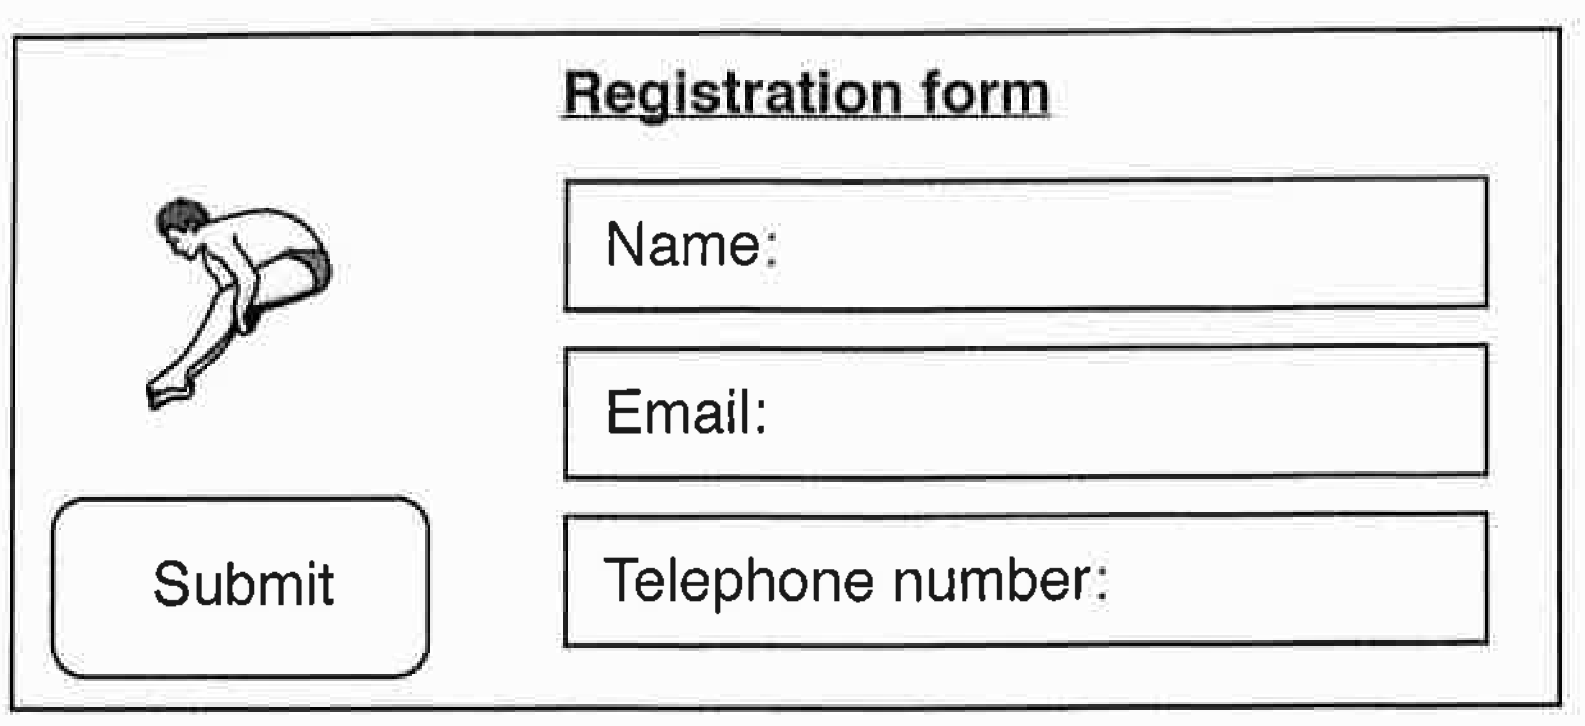
\includegraphics[width=0.5\paperwidth]{C:/Users/Admin/Desktop/Github/question_bank/LyX/static/img/9597-ALVL-2018-P2-Q6-2}
\par\end{center}

Explain how the web server will use server-side script to process
this form. \hfill{} {[}5{]}
\item The organisers of the championship store all the data for the event
using cloud storage. 

Describe\textbf{ three} economic benefits to the organisers of using
cloud-based storage. \hfill{}{[}3{]}
\end{enumerate}
{[}SPLIT\_HERE{]}
\end{enumerate}

\end{document}
